\chapter{Fundamentação Teórica}

Para uma série de aplicações, a maneira mais adequada de se obter imagens da superfície de um objeto cilíndrico é adquirir fotografias dessa superfície a partir de diferentes ângulos e, posteriormente, realizar a união destas imagens através de algoritmos de registro utilizados em imagens panorâmicas e outros tipos de mosaicos de imagens \cite{Park:2013}. 
Com a intenção de diminuir deformações causadas pelas distorções projetivas, bem como pelas diferentes perspectivas de projeção geradas pela geometria tridimensional do objeto de interesse, em \cite{Lin:2013} é proposto um algoritmo que corrige essas distorções, utilizando técnicas de trigonometria que proporcionam a identificação de uma coordenada específica da imagem  que representa uma distorção por ângulo. Estes pontos são submetidos a uma transformação geométrica de acordo com a sua posição na imagem.  Neste capítulo, o método proposto em \cite{Lin:2013}, bem como sua aplicação, é detalhado.

\section{Construção das imagens}

A solução proposta em \cite{Lin:2013} se baseia na fusão de imagens obtidas através de ângulos distintos, a fim de ilustrar diferentes regiões da superfície de um cilindro. A Figura~\ref{fig:cameras} representa uma vista superior da disposição entre a garrafa e as quatro câmeras posicionadas com o objetivo de garantir uma visão completa do perímetro do objeto.  

\begin{figure}[ht]
    \caption{Vista superior da disposição das câmeras.}
    \centering
     \vspace{0.4cm}
    \begin{minipage}{.5\textwidth}
        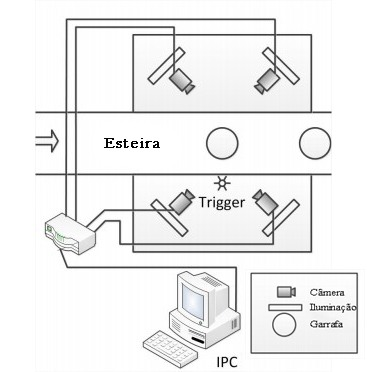
\includegraphics[width=\linewidth]{TCC/Imagens/cameras.jpg}
        \fonte{Adaptado de Lin et al. (2013).}
	\end{minipage}
    \label{fig:cameras}
\end{figure}


Neste sistema, uma esteira realiza o movimento da garrafa que, quando posicionada em frente ao \textit{trigger}, dispara o comando de captura fazendo com que todas as imagens sejam obtidas simultaneamente. Por fim, estas imagens são enviadas ao IPC (\textit{Industrial Personal Computer}) que é responsável por processá-las.

Basicamente, três tipos de distorções são encontradas em imagens adquiridas no contexto deste sistema. O primeiro corresponde às distorções projetivas geradas pelo desalinhamento do plano do sensor com o plano da imagem (cena). O segundo diz respeito às distorções projetivas causadas pela projeção de um objeto (cena) tridimensional em um plano (sensor de aquisição). O terceiro diz respeito às distorções geradas pelo conjunto óptico, principalmente as distorções geométricas geradas pela objetiva. O primeiro tipo de distorção é tratado em \cite{Lin:2013} por meio da  biblioteca de calibração \textit{Camera Calibration Toolbox} do Matlab\textsuperscript{\tiny\textregistered} \cite{CameraCalibration}. Visando a avaliação de uma solução que dispense processos elaborados de calibração, neste trabalho, a compensação desse tipo de distorção é negligenciada. O mapeamento das demais distorções é abordado na seção seguinte.

\subsection{Projeções cilíndricas}

A projeção de um objeto (aproximadamente) cilíndrico no plano do sensor gera distorções nas direções vertical e horizontal. É possível dizer que todas as representações de superfícies curvas em um plano envolvem “contrações” ou “extensões” que podem resultar em distorções ou “rasgos” na tentativa de corrigir estes artefatos através de compensações  geométricas \cite{Shen:2013}. Diferentes técnicas de identificação e representação dessas distorções são utilizadas no sentido de se alcançar resultados que possuam certas propriedades favoráveis para um propósito específico \cite{Shen:2013, Zhao:2013}. 

\begin{figure}[ht]
    \caption{Diagrama esquemático da distorção causada no eixo horizontal.}
    \centering
    \vspace{0.4cm}
    \begin{minipage}{.3\textwidth}
         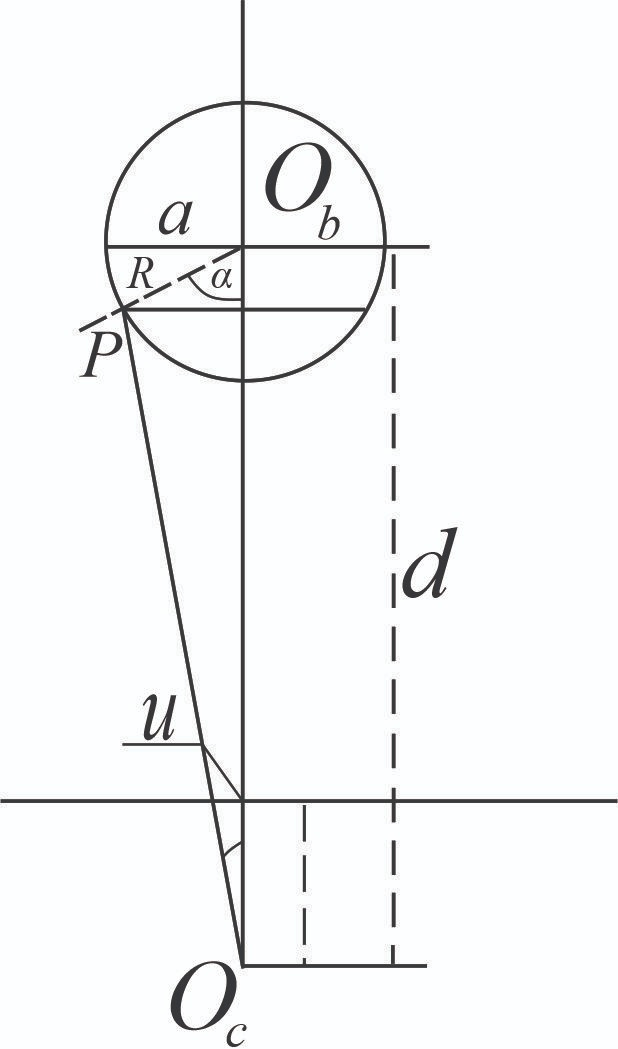
\includegraphics[width=\textwidth]{TCC/Imagens/dist_horz_2.jpeg}
         \fonte{Adaptado de Lin et al. (2013).}
	\end{minipage}
    \label{fig:dist_horz}
\end{figure}


A fim de obter as coordenadas que mapeiam a distorção do eixo $x$ (horizontal), em \cite{Lin:2013} foi considerado o diagrama esquemático apresentado na Figura~\ref{fig:dist_horz}. Nesse diagrama, $u$ representa a coordenada $x$ do ponto $P$ e $\alpha$ denota o ângulo entre os segmentos de reta   $\overline{O_{b}P}$ e $\overline{O_{b}O_{c}}$.  Observando o diagrama é possível estabelecer, através de relações trigonométricas, a função que representa as distorções horizontais, dada por

\begin{equation}
    u = a \frac{\sqrt{d^2 - R^2} \sin{(\alpha)}}{d - R\cos{ \left (\alpha \right)}}
    \label{equacao:dist_horz} 
\end{equation}
em que $R$ é o raio do cilindro (garrafa), $a$ é a distância entre o ponto extremo horizontal (da garrafa) e o seu respectivo centro (na imagem) e $d$ é a distância entre o centro óptico da câmera, $O_{c}$, e o centro da garrafa, $O_{b}$. Levando em consideração que calibrações intrínsecas à câmera estão sendo negligenciadas (não permitindo o real dimensionamento do ângulo máximo real alcançado pelo sensor), neste trabalho o limite lateral esquerdo da garrafa será considerado ideal, representando -90$^\circ$ enquanto o seu ângulo de meia volta identifica o limite à direita do rótulo.

\iffalse
Olha, estive procurando alguns nortes com relação a essa questão da causa desta distorção vertical... Quando se trata de distorção diretamente da lente, acontece o "barrel effect", onde a distorção também deveria ser causada pelos lados..
Alguns sites (não achei nada cientificamente apontado pra isso) demonstram a característica de elipse de acordo com o ponto de visão no objeto cilindrico:
http://kaplanpicturemaker.com/perspective/cylinders (up and around)
https://ariartlessons.wordpress.com/2012/06/12/cylinders-in-perspective/

Aqui os autores do site comentam que esse efeito é causado pela perspectiva, assim como quando desenhamos um cilindro em isometrica, a parte inferior tem o traço de uma elipse na parte inferior. Pelo que eu entendi, caso a foto seja tirada de uma distancia maior, esse efeito pode vir a desaparecer por completo (diminuindo o angulo vertical entre o sensor da câmera e o ponto de maior ordenada da garrafa). Infelizmente eu não sei o que afirmar aqui, na minha interpretação, acaba sendo uma questão de perspectiva.

não sei se poderia referenciar isso sem um embasamento sólido em qualquer um dos casos

\fi
 
Em \cite{Lin:2013} as distorções geradas pela a \iffalse curvatura da lente e pela\fi perspectiva da cena em relação ao eixo vertical são modeladas como uma elipse, assim como é ilustrado na Figura~\ref{fig:dist_vert}, onde a Figura~\ref{fig:dist_vert}~(a) representa o rótulo ideal (sem distorções verticais) e a Figura~\ref{fig:dist_vert}~(b) demonstra o efeito da distorção causado na fotografia. Na imagem em que o rótulo não apresenta distorções, é possível observar que apesar de todos os pontos entre $P_{a}$ e $P_{b}$ terem a mesma ordenada a distorção projetiva causa uma forma geométrica distinta ao plano da imagem obtida, representada no diagrama ao lado. Na figura distorcida, nota-se que quando o ponto se encontra acima do ponto central da imagem, a elipse tem o segmento de curva para cima e quando o ponto se encontra abaixo, tens o segmento inferior da elipse. Na Figura~\ref{fig:dist_vert}~(b) os pontilhados auxiliam na visualização da forma geométrica completa da elipse.


\begin{figure}[ht]
    \caption{Diagrama da distorção vertical. (a) Imagem sem a distorção; (b) Imagem distorcida.}     
    \centering
    \vspace{0.3cm}
    \begin{minipage}{.5\textwidth}
      \centering
            \begin{tabular}{cc}
            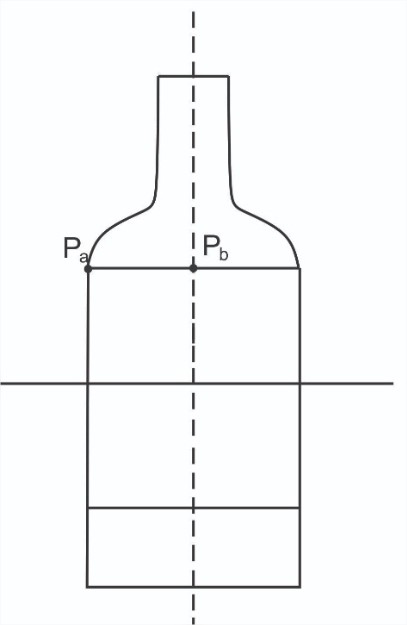
\includegraphics[width=.5\linewidth]{TCC/Imagens/dia_vert_plan.jpg} 
            &
            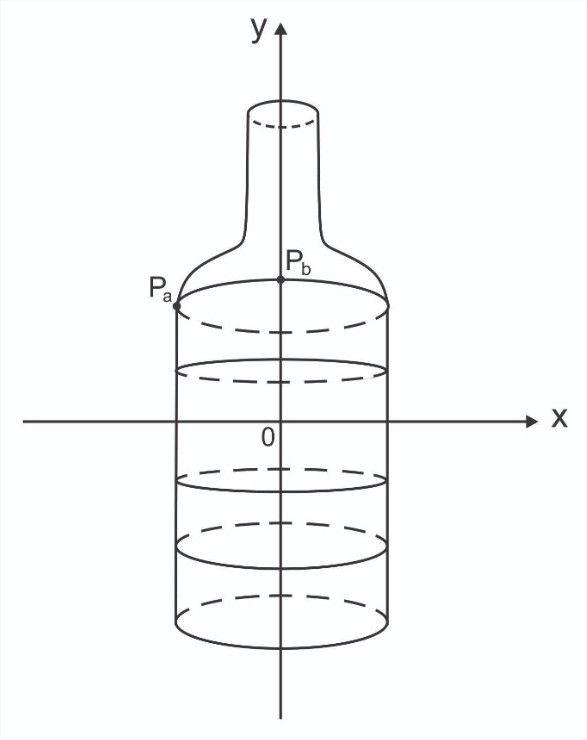
\includegraphics[width=.55\linewidth]{TCC/Imagens/diag_vert_dist.jpg}
            \\
            (a) & (b)
            \end{tabular}
        \fonte{O autor (2020).}
	\end{minipage}
    \label{fig:dist_vert}
\end{figure}

 
Para um melhor entendimento da equação que representa as distorções verticais, se vê necessária uma breve abordagem na equação fundamental que representa a elipse no plano cartesiano (ver Figura~\ref{fig:ellipse_imagem}). Em geometria, uma elipse é um tipo de seção cônica, isto é, caso uma superfície cônica seja cortada por um plano que não passe pela sua base e que não ultrapasse as duas folhas do cone, a interseção entre o cone e o plano é uma elipse. As medidas da elipse são dadas pela metade dos eixos maior e menor sendo chamadas, respectivamente, de semi-eixo maior ($a$) e semi-eixo menor ($b$). A equação fundamental da elipse é dada por

\begin{equation}
    \frac{x^2}{a^2} + \frac{y^2}{b^2} = 1
    \label{equacao:ellipse}
\end{equation}

\begin{figure}[htb]
    \caption{Forma geométrica de uma elipse representada no plano cartesiano.}
    \centering
    \begin{minipage}{.5\textwidth}
      \centering
         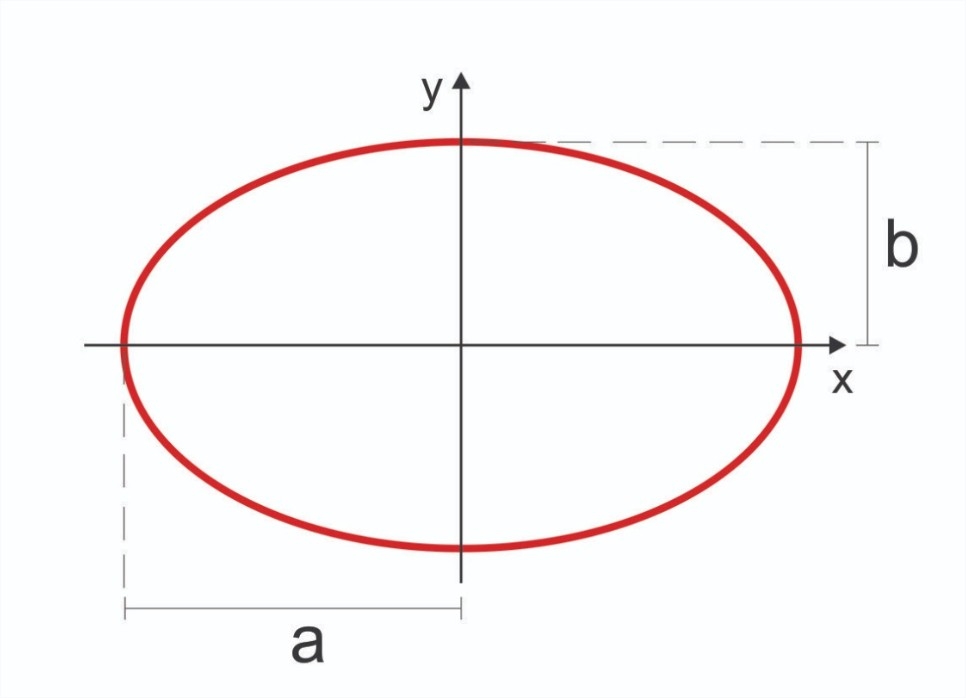
\includegraphics[width=.95\linewidth]{TCC/Imagens/ellipse_imagem.jpg}
         \fonte{O autor (2020).}
	\end{minipage}
    \label{fig:ellipse_imagem}
\end{figure}

Com isso, \citet*{Lin:2013} mapeiam as distorções verticais através da equação descrita a seguir:

\begin{equation}
    %b\sqrt{1 - \frac{u^2}{a^2}} =
    v = h \frac{R}{d+R} \sqrt{1 - \frac{(d^2 - R^2)\sin^2{(\alpha)}}{[d - R\cos{ (\alpha)}]^2}}
    \label{equacao:dist_vert}
\end{equation}
em que $h$ representa a distância entre o centro do rótulo e sua ordenada máxima (na imagem), chamada de $v_{max}$. Uma representação da elipse que identifica uma distorção vertical pode ser vista na Figura~\ref{fig:bottle_ellipse}.


\begin{figure}[htb]
    \caption{Forma geométrica de uma elipse representando a distorção do eixo vertical.}
    \centering
    \vspace{0.3cm}
    \begin{minipage}{.5\textwidth}
      \centering
         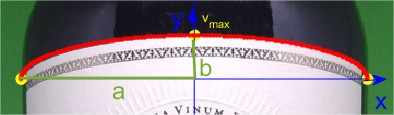
\includegraphics[width=.95\linewidth]{TCC/Imagens/ellipse_apre.jpg}
         \fonte{O autor (2020).}
	\end{minipage}
    \label{fig:bottle_ellipse}
\end{figure}

Com as coordenadas $u$ e $v$ que representam as distorções horizontais e verticais respectivamente identificadas, é possível expandir (realizar as compensações geométricas) a imagem a partir dos pontos mapeados pelo ângulo $\alpha$. Realizando este procedimento com cada uma das imagens, serão formadas no total quatro novas imagens planificadas que, ao se unirem, representarão o perímetro total da garrafa.

\subsection{Compensações geométricas}

Em \cite{Lin:2013} não é detalhado o método adotado para realizar as compensações geométricas. Portanto, nesta revisão são consideradas transformações geométricas a partir do mapeamento das distorções identificadas na imagem. Segundo \cite{Gonzales:2000}, uma transformação geométrica consiste na operação de uma transformação espacial na imagem, sendo essa, responsável pela ''reorganização'' dos pixeis através de regras pré-estabelecidas. Para deixar o procedimento mais claro, será mencionado o exemplo utilizado em \cite{Gonzales:2000}:

Supondo que uma imagem denominada $f$ com coordenadas de pixeis definidas por $(x,y)$ seja submetida a uma transformação geométrica para se tornar uma nova imagem $g$, onde suas novas coordenadas serão dadas por $(x',y')$, a transformação é dada pela seguinte notação:

\begin{equation}
    \begin{array}{l}
        x'= r(x,y) \\
        y'= s(x,y)
    \end{array}
\end{equation}
em que $r(x,y)$ e $s(x,y)$ são as transformações que produzem uma nova imagem $g(x', y')$. Por exemplo, se $r(x,y) = {x}/{2}$ e $s(x,y) = {y}/{2}$, a distorção pode ser descrita como um ``achatamento'' de $f(x, y)$, reduzindo seu tamanho pela metade em ambos os eixos.

O método mais utilizado para modelar essa transformação é a seleção de \textit{tiepoints}, que são coordenadas conhecidas na imagem distorcida e na imagem original \cite{Gonzales:2000}. Na Figura~\ref{fig:spatial_transform_gonzales} é possível visualizar um paralelogramo (figura distorcida) e um quadrado (figura corrigida), onde os \textit{tiepoints} são destacados pelos vértices.

\begin{figure}[htb]
    \caption{Pontos correspondentes em diferentes segmentos de imagem.}
    \centering
    \begin{minipage}{.5\textwidth}
      \centering
         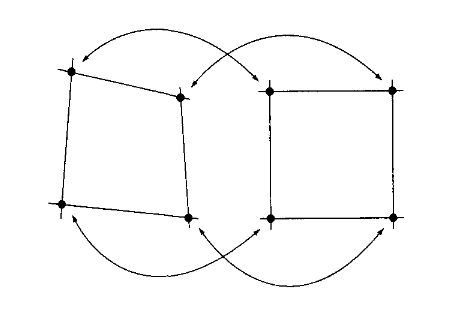
\includegraphics[width=1\linewidth]{TCC/Imagens/spatial_transform.png}
         \fonte{Gonzales e Woods (2000).}
	\end{minipage}
    \label{fig:spatial_transform_gonzales}
\end{figure}


Uma (matriz de) transformação comumente utilizada e que é consistente com o problema abordado neste trabalho é a (matriz de) transformação projetiva. Essa transformação, causa o efeito de inclinação sob o plano da imagem, onde normalmente as linhas paralelas convergem para um ''ponto de fuga'' (ver Figura~\ref{fig:projective_transf}). A equação que descreve uma transformação geométrica na imagem é dada por \cite{Wolberg:1990} como

\begin{equation}
    [x',y',w'] = [u, v, w]  \mathbf{T}
    \label{equacao:matriz_transform}
\end{equation}
em que
\begin{equation}
    \mathbf{T} = 
    \begin{bmatrix}
    a_{11} &  a_{12} & a_{13} \\
    a_{21} &  a_{22} & a_{23} \\
    a_{31} &  a_{32} & a_{33}
    \end{bmatrix}
    \nonumber
\end{equation}
e $[x',y',w']$ é a coordenada homogênea\footnote{Coordenadas homogêneas são um sistema de coordenadas utilizadas em geometria projetiva, assim como coordenadas cartesianas são utilizadas em geometria Euclidiana. A vantagem delas é que pontos, incluindo pontos no infinito, podem ser representados por coordenadas finitas. Formulações que envolvem coordenadas homogêneas são geralmente mais simples e simétricas que as respectivas formulações para coordenadas cartesianas. \cite{August:1997}} de $\mathbf{p} = [x ,y]$.

Diferente de uma transformação afim (mudança de escala, movimento de rotação ou translação), os valores da última coluna são diferentes de zero \cite{Wolberg:1990}. Portando, $a_{13}$ e $a_{23}$ influenciam diretamente no ``ponto de fuga'', de maneira que, quanto maiores são os seus valores, mais o ponto de fuga se aproxima da origem e, portanto, as linhas paralelas parecem convergir mais rapidamente, proporcionando uma inclinação maior no plano da imagem, causando uma ''sensação'' de profundidade na cena (ver Figura~\ref{fig:projective_transf}. Portanto, o mapeamento (fora da forma homogênea) entre a imagem transformada e a imagem original é dado por
 
 \begin{equation}
    \begin{array}{l}
        x = \frac{x'}{w'} = \frac{a_{11}u + a_{21}v+ a_{31}}{a_{13}u + a_{23}v+ a_{33}} \\
        \\
        y = \frac{y'}{w'} = \frac{a_{12}u + a_{22}v+ a_{32}}{a_{13}u + a_{23}v+ a_{33}}
    \end{array}
    \label{equacao:map_transform}
\end{equation}

\begin{figure}[htb]
    \caption{Demonstração de uma transformada geométrica projetiva.}
    \centering
    \begin{minipage}{.9\textwidth}
        \centering
        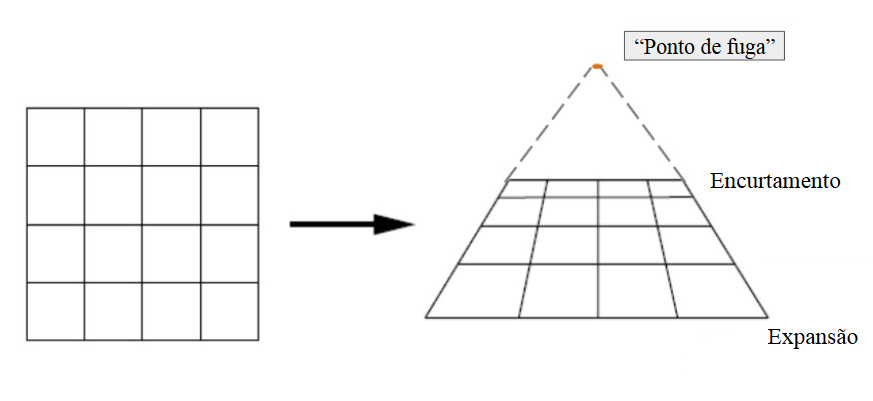
\includegraphics[width=\textwidth]{TCC/Imagens/transform.jpg}
         \fonte{O autor (2020).}
	\end{minipage}
    \label{fig:projective_transf}
\end{figure}


% Em \cite{Wolberg:1990} é afirmado que o mapeamento projetivo inverso é calculado diretamente em termos da matriz inversa de $T$. Portanto, a maneira mais fácil de transformar o plano distorcido em um plano retificado (um paralelogramo para um retângulo, por exemplo) e com a utilização da equação \ref{equacao:inverse_transform}.

% \begin{equation}
%   T^{-1} = \frac{adj(T)}{det(T)}
%     \label{equacao:inverse_transform}
% \end{equation}

% em que $adj(T)$ é a matriz adjunta e $det(T)$ é a sua determinante.\\

Observando que a matriz $\mathbf{T}$ possui dimensões $3\times3$, é possível afirmar que sua normalização resulta em $a_{33}$ = 1, garantindo oito ``termos livres'' na matriz. Com isso, é possível estabelecer uma transformação geométrica projetiva a partir dos quatro pontos conhecidos (\textit{tiepoints}) na imagem original e quatro pontos na imagem distorcida.

Pode-se ressaltar a afirmação de \cite{Gonzales:2000} novamente, em que a utilização de \textit{tiepoints} para modelar a transformação entre ambas as imagens pode ser estabelecida. Em \cite{Wolberg:1990} e \cite{Heckbert:1989} os autores exploram a fundo métodos que aceleram os procedimentos de transformada geométrica, considerando comportamentos conhecidos entre as coordenadas das imagem distorcida e da imagem retificada e melhoria de desempenho, entre outros fatores.

\iffalse
R. Gonzalez, “Digital Image Processing,” Section 5 11 Section 5.11
George Wolberg, Digital Image Warping, Wiley-IEEE Computer Society Press, 1990
\fi

\subsection{Mosaico de imagens}

A construção de uma imagem panorâmica é uma técnica que reúne múltiplas imagens adquiridas a partir de diferentes vistas. O principal objetivo é formar uma imagem única e abrangente, também chamada de mosaico \cite{Shum:2000}. Para que o mosaico tenha uma qualidade considerável, a união das imagens (também conhecida por ``fusão'') é um dos passos mais importantes. Esse tipo de técnica se baseia em premissas matemáticas que demandam, por exemplo, a existência de semelhanças e sobreposições consideráveis entre regiões das diferentes imagens a serem fundidas. Entretanto, é comum que ocorram variações geométricas nas áreas de sobreposição das imagens ou violações nessas premissas durante o processo de aquisição, acarretando em artefatos degradantes, como regiões desfocadas ou costuras visíveis entre as imagens \cite{Gracias:2009}.

Em \cite{Levin:2004}, as técnicas de mosaico são divididas em duas abordagens: suavizações entre transições; e localizações ideais de costura. O trabalho proposto em  \cite{Lin:2013} segue a segunda abordagem, visando obter um resultado mais preciso na união das imagens. Dessa forma, foi empregada uma técnica de registro de imagens que permite contornar os problemas de mudança de escala, variações de iluminação e 
a possibilidade da garrafa ser apresentada para as câmeras rotacionada (em diferentes posições angulares). Dentre as diversas técnicas disponíveis para a detecção de características comuns entre imagens em \cite{Lin:2013} foi utilizado o método SIFT (\textit{Scale-invariant feature transform}), este, pode ser considerado como uma espécie de detector de bordas/linhas que apresentam características padrões na imagem  \cite{Lowe:2001}. Segundo \cite{Mikolajczyk:2005}, o algoritmo SIFT é um dos métodos que obtêm os melhores resultados de correspondência entre pontos, levando em consideração os problemas mencionados.

Em cada uma das imagens, já com as distorções compensadas, o algoritmo é utilizado a fim de identificar \textit{key points} (também chamados de \textit{pontos descritores}, em português), estes pontos são responsáveis pela identificação das bordas mais relevantes da imagem (normalmente baseados em uma frequência). Na Figura~\ref{fig:SIFT} é possível visualizar uma imagem com seus \textit{key points} destacados em vermelho. 

Em pares, as imagens são submetidas a um processo de comparação entre seus respectivos \textit{key points}, identificando características em comum entre os pontos descritores de ambas. Os pontos descritores que tem a maior taxa de similaridade entre si (pixels vizinhos que apresentam o mesmo padrão, por exemplo) são considerados o mesmo ponto no espaço, ou seja, o ponto ideal de costura entre as imagens. Para a realização dessa tarefa, é necessário gerar uma matriz de homografia.

\begin{figure}[htb]
    \caption{Destaque dos \textit{key points} da imagem, obtidos com a utilização do SIFT.}
    \label{fig:SIFT}
    \centering
	\vspace{0.4cm}
	\begin{minipage}{.7\textwidth}
	    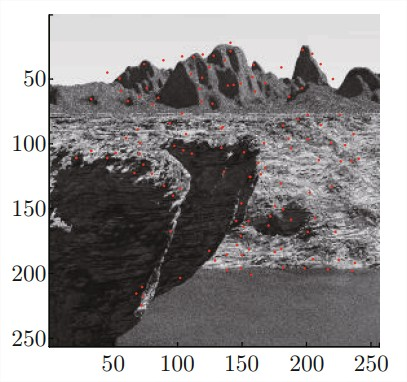
\includegraphics[width=\textwidth]{TCC/Imagens/SIFT.jpg}
	    \fonte{Wang et al. (2017).}
	\end{minipage}
\end{figure}

Em \cite{Gledhill:2003} uma matriz de homografia é definida como um mapeamento entre duas imagens de uma superfície planar, constituindo uma única cena, adquiridas de perspectivas diferentes. Ou seja, duas imagens de uma mesma cena estão relacionadas por uma matriz de homografia (normalmente de dimensão $3\times3$, representando escala, rotação e translação entre as imagens). Essa matriz pode ser utilizada para remapear as imagens a partir de diferentes planos. Na Figura~\ref{fig:RANSAC_OUTLIER} é possível observar o resultado da correspondência de características (obtidas através do SIFT) entre imagens da mesma cena, obtidas de planos distintos.

\begin{figure}[htb]
    \caption{Exemplo de correspondência entre pontos com a utilização do SIFT. }
    \centering
    \vspace{0.3cm}
    \begin{minipage}{.9\textwidth}
         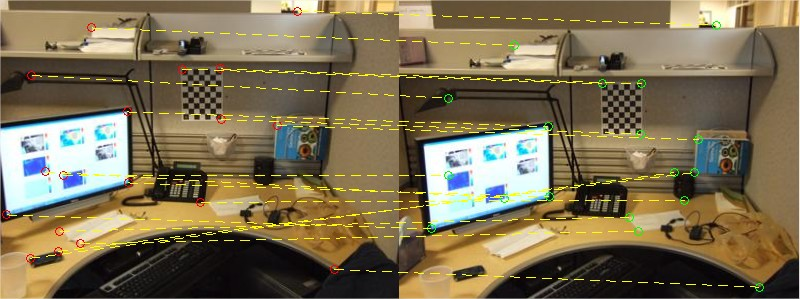
\includegraphics[width=\textwidth]{TCC/Imagens/RANSAC_OUTLIERS.jpg}
         \fonte{\cite{RANSAC}.}
	\end{minipage}
    \label{fig:RANSAC_OUTLIER}
\end{figure}

A fim de evitar problemas de registro, é necessário verificar se pontos de correspondência não foram estimados incorretamente. Para isso, é utilizado o algoritmo RANSAC (\textit{Random Sample Consensus}), que é um método iterativo para estimar um modelo matemático de um conjunto de dados que contém pontos que fogem do
padrão estatístico, chamados de \textit{outliers}, e pontos que estão dentro deste padrão, denominados \textit{inliers} \cite{Fischler:1981}. Com a classificação desses dados
concluída, é possível gerar uma nova matriz de homografia considerando apenas as coordenadas em ambas as imagens que estejam dentro do modelo matemático gerado. A remoção 
dos \textit{outliers} é demonstrada na Figura~\ref{fig:RANSAC_INLIERS}, melhorando consideravelmente a taxa de acerto na correspondência entre pontos nas duas imagens.

\begin{figure}[htb]
    \caption{Remoção dos \textit{outliers} com a utilização do RANSAC. }
    \centering
    \vspace{0.3cm}
    \begin{minipage}{.9\textwidth}
         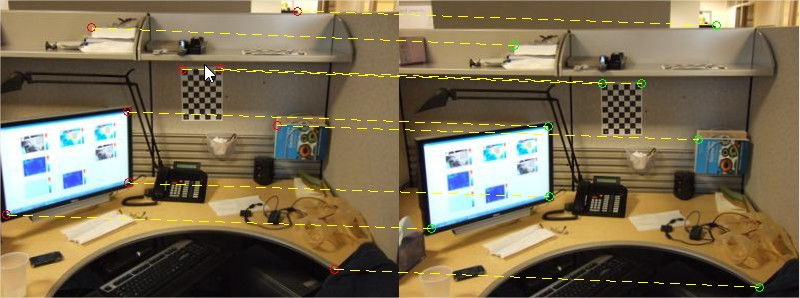
\includegraphics[width=\textwidth]{TCC/Imagens/RANSAC_INLIERS.jpg}
         \fonte{\cite{RANSAC}.}
	\end{minipage}
    \label{fig:RANSAC_INLIERS}
\end{figure}


Finalmente, com a melhor matriz de homografia definida, agora é possível realizar a fusão deste par de imagens. Em \cite{Lin:2013}, os autores não mencionam o método que utilizaram 
para realizar a fusão das imagens, todavia é necessário utilizar algum método para corrigir artefatos que são causados pela sobreposição das imagens unidas. Realizando a união de todas as imagens, é possível visualizar todo o perímetro da garrafa com uma única imagem.


